\documentclass[../../Main/Main.tex]{subfiles}
\begin{document}

\chapter{Statistical mechanics and phase transitions}

\section{Statistical mechanics of phase transitions}

From the microscopic degrees of freedom, one compute the partition function in the appropriate ensemble, then the corresponding thermodynamic potential and from it all the thermodynamic properties of the system as \emph{equilibrium phases} and, if present, \emph{phase transitions}. Actually, until the '30 there were strong concerns about the possibility that statistical mechanics could describe phase transitions.

\begin{figure}[h!]
\begin{minipage}[c]{0.5\linewidth}
\centering
\subfloat[][Region \( \Omega  \) with boundary \( \partial{\Omega }  \).]{
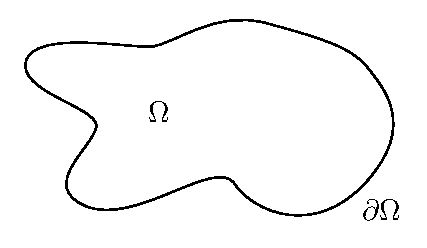
\includegraphics[width=0.8\textwidth]{./img/2__1.pdf}
    \label{fig:5_1_0} }
\end{minipage}
\begin{minipage}[]{0.5\linewidth}
\centering
\subfloat[][Magnetic system with characteristic length \emph{L}.]{
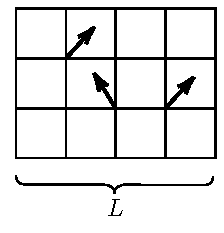
\includegraphics[width=0.5\textwidth]{./img/3__1.pdf}
    \label{fig:5_1_1} }
\end{minipage}
\caption{\label{fig:} }
\end{figure}


Let us consider a system withing a region \( \Omega  \) of volume \( V(\Omega ) \) and boundary \( \partial{\Omega }  \)    of area \( S (\Omega ) \). Denoting by \emph{L} a characteristic lenght of the system

\begin{equation*}
  V(\Omega ) \propto L^d, \quad S(\Omega  ) \propto L^{d-1}
\end{equation*}
where \emph{d} is the spatial dimension where the system is embedded.
\begin{remark}
Space \( \Omega  \) can be either \emph{discrete} or \emph{continuous}.
\end{remark}
Suppose that the system is \emph{finite}. Formally, we can write
\begin{equation}
  \mathcal{H}_{\Omega } = - \sum_{n}^{} k_n \Theta _n
\end{equation}
where
\begin{itemize}
  \item \( k_n \): are the coupling constants. In general, but not always, they are proportional to the  \emph{intensive thermodynamic variables}.
  \item \( \Theta _n \): is a linear, or higher order, combination of the dynamical microscopic degrees of freedom (local operators in quantum statistical mechanics).
  \item \( k_n \Theta _n \): must obey the symmetry of the system. It is important that in principle the term satisfies the symmetry of the system. This is a master rule!
\end{itemize}

\begin{remark}
The symmetry of the system is related to the space of degrees of freedom, which in general is different from the embedding space \( \Omega  \).
\end{remark}

To fix the idea, let us consider two classical examples: the magnetic system and the fluid system.

\subsection{Magnetic system (canonical)}
The degrees of freedom are the \emph{spins} lying on a Bravais lattice \( \va{S_i}  \), with \( 1 \le i \le N(\Omega ) \), where the \( N(\Omega )   \) are the number of lattice sites. A configuration is the orientation of the spin in each site \( \mathcal{C} = \{ \va{S_1},\dots,\va{S_N} \}  \).
We have:
\begin{subequations}
\begin{align}
  \Theta _1 &=  \sum_{i}^{} \va{S_i} \\
  \Theta _2 &= \sum_{ij}^{} \va{S_i} \vdot \va{S_j}
\end{align}
\end{subequations}
We consider the trace operation, that is the sum over all possible values that each degree of freedom can assume:
\begin{equation}
  \Tr \equiv \sum_{\{ \mathcal{C} \}  }^{}  \equiv \sum_{\va{S_1} }^{} \sum_{\va{S_2} }^{} \dots  \sum_{\va{S_N} }^{}
\end{equation}
where \( \sum_{}^{}   \) can also indicate an integration if values are continuous.

The \emph{canonic partition function} is
\begin{empheq}[box=\myyellowbox]{equation}
  Q_ \Omega (T, \{ k_n \} ) = \Tr( e^{-\beta \mathcal{H }_ \Omega} )
\end{empheq}
with \( \beta \equiv \frac{1}{k_B T} \).
\subsection{Fluid system (gran canonical)}
Consider \emph{N} particles in a volume \emph{V}, with number density \( \rho =N/V \).
The \( 2dN \)  degrees of freedom are
\begin{equation*}
  \{ \mathcal{C} \} =  \{ (\va{x_i}, \va{p_i}  )_{i=1,\dots,N} \}
\end{equation*}
and
\begin{subequations}
\begin{align}
  \Theta _1 &= \sum_{i}^{} \qty[\frac{\va{ p_i}^2}{2 m_i} + U_1 (\va{x_i} )]    \\
  \Theta _2 &= \frac{1}{2} \sum_{i>j}^{} U (\abs{\va{x_i}-\va{x_j}  } )
\end{align}
\end{subequations}
The trace operation is
\begin{equation}
  \Tr \equiv \sum_{\{ \mathcal{C} \}  }^{} = \sum_{N=0}^{\infty } \frac{1}{N!} \int_{}^{} \prod_{i=1}^{N} \frac{ (\dd[]{\va{p_i} }  ) (\dd[]{\va{x_i} } )}{h^{dN}}
\end{equation}
The \emph{gran canonical partition function} is:
\begin{empheq}[box=\myyellowbox]{equation}
  \mathcal{F}_ \Omega = \Tr(e^{-\beta (\mathcal{H}_ \Omega - \mu N) } )
\end{empheq}

For a generic partition function \( Q_ \Omega (T, \{ k_n \}  ) \), we can define the finite system \emph{free energy} as
\begin{empheq}[box=\myyellowbox]{equation}
  F_ \Omega [T,\{ k_n \}  ] = - k_B T \ln{Q_ \Omega (T, \{ k_n \}  )}
\end{empheq}
The relation with thermodynamic is trough the \emph{theromdynamic limit}. 

Since the free energy is an extensive function,
\begin{equation*}
  F_ \Omega \propto V (\Omega)  \sim L^d
\end{equation*}
In general, one can write
\begin{empheq}[box=\myyellowbox]{equation}
  F_ \Omega [T,\{ k_n \}  ] = V (\Omega ) f_b [T,\{ k_n \}  ] + S (\Omega ) f_s [T,\{ k_n \}  ] + O (L^{d-2})
\end{empheq}
where \( f_b [T,\{ k_n \}  ] \) is the bulk free energy density.

  \begin{definition}{Bulk free energy density}{}
  We define the \emph{bulk free energy density} as
  \begin{equation}
    f_b [T,\{ k_n \}  ] \equiv \lim_{V (\Omega ) \rightarrow \infty } \frac{F_ \Omega [T,\{ k_n \}  ]}{V (\Omega )}
  \end{equation}
  if the limit exists (to prove for each system) and does not depend on \( \Omega  \).
  \end{definition}


For a system defined on a lattice we have
\begin{equation*}
  L (\Omega ) \propto N (\Omega )^{1/d}, \quad V (\Omega ) \propto N (\Omega )
\end{equation*}
\begin{equation*}
  f_b [T,\{ k_n \}  ] = \lim_{N (\Omega) \rightarrow \infty } \frac{1}{N (\Omega )} F_N [T,\{ k_n \}  ]
\end{equation*}
To get information on surface property of the system, let us calculate
\begin{equation}
  f_s [T,\{ k_n \}  ] \equiv \lim_{S (\Omega ) \rightarrow \infty } \frac{F_ \Omega [T,\{ k_n \}  ]  - V (\Omega ) f_b [T,\{ k_n \}  ]}{S (\Omega )}
\end{equation}

\subsection{Partition Function as Generating Function}

Given the canonical partition function:
\begin{equation}
  Z[T, \set{ k_{m} }] = \Trace_{ \set{ C }} e^{-\beta E(C)}
\end{equation}

we can compute the thermal averages at equilibrium as derivatives of $Z$. For instance the average of the energy \( \langle \frac{1}{Z}\Tr \rangle [E(C) \exp(-\beta E(C))] \)

%%%%%%QUI INSERISCI PARTE 1%%%%%%



\subsection{Thermodynamic limit with additional constraints}
For a fluid we cannot simply take the limit \( V (\Omega ) \rightarrow \infty  \) by keeping \( N \) fixed, otherwise we will always get a infiinite system with \emph{zero density}. One has to take also the limit \( N(\Omega ) \rightarrow \infty  \) such that:
\begin{equation*}
  \frac{N (\Omega )}{V (\Omega )} \equiv \rho = const
\end{equation*}
In general, is not so easy to prove the existence of the limit and it depends on the range of the particle-particle interactions.

\subsection{Statistical mechanics and phase transitions}
Since all the thermodynamic information of a system can be obtained by the partition function, in principle, also the ones concerning the existence and nature of the phase transition must be contained in \emph{Z} (or \emph{Q}). On the other hand, we know from thermodynamic that phase transitions are characterized by singularities in the derivation of \emph{F}. Also \emph{Z} must display these singularities.

On the other hand, \emph{Z} is a sum of exponentials
\begin{equation}
  Z_ \Omega = \Tr(e^{-\beta \mathcal{H}_ \Omega } )
\end{equation}
the exponentials are analytic functions everywhere (they converge), hence \( Z_ \Omega  \) is analytic for \( \Omega  \) finite!

The question is: where do singularities come from?
It is only in the thermodynamic limit that singularities in \emph{F} and hence points describing phase transitions can arise!

For summarizing, there is no way out of this for producing singularities. The singularities will develop in the thermodynamic limits. For reaching singularities, we have to reach so precision in thermodynamic that we are not able to go exactly into the critical point. How can we relate singularities, geometrically, in the behaviour of the system?

 \section{Critical point and correlations of fluctuations}
 From thermodynamics, we know that, at the critical point, some response functions may diverge. Now, we show that this is a consequence of the onset of microscopic fluctuactions that are spatially correlated over long distances.
 To see this, let us compute the response of a ferromagnetic in presence of an external magnetic field \emph{H}.
 The Gibbs partition function of a generic magnetic system is as equation:
 \begin{equation*}
   Z_{\text{Gibbs}} [T,\{ k_n \}  ] = \Tr(e^{-\beta (\mathcal{H} (\mathcal{C}) - H M (\mathcal{C}))} ) = \sum_{M,E}^{} e^{-\beta E + \beta H M} \Omega (E,M)
 \end{equation*}
\begin{remark}
The term \( (- H M) \) is the work done by the system against the external field \emph{H} to mantain a given magnetization \( M \).
\end{remark}
\begin{equation}
  \expval{M} = \eval{ \pdv{\ln{Z_G} }{(\beta H)} }_T = \frac{1}{Z_G} \Tr[M (\mathcal{C}) e^{-\beta ( \mathcal{H} (\mathcal{C}) - H M (\mathcal{C}))} ]
\end{equation}
\begin{equation}
  \chi _T = \pdv{\expval{M} }{H} = \qty{\frac{\beta }{Z_G} \Tr \qty[M^2 (\mathcal{C}) e^{-\beta \mathcal{H} + \beta H M} ] - \frac{\beta }{Z_G^2} \qty[ \Tr \qty[M (\mathcal{C}) e^{-\beta \mathcal{H} + \beta H M } ]  ]^2 }
\end{equation}
Hence,
\begin{equation}
  \chi _T = \frac{1}{k_B T} \qty(\expval{M^2} - \expval{M}^2  )
\end{equation}
\emph{The thermodynamic response function \( \chi _T \) in statistical mechanics is related to the variance of the magnetization}.

We can relate the above expression with the correlation of the microscopic by performing a coarse-graining of the system, where the magnetization \( M (\mathcal{C}) \)  can be computed  as an integral
\begin{equation}
  M (\mathcal{C}) = \int_{}^{} \dd[3]{\va{r}}   m (\va{r})
\end{equation}
where $m (\va{r}$ is defined through a coarse graining approach as the local average on a block of an infinitesimal subsystem.
Hence,
\begin{equation}
  k_B T \chi _T = \int_{}^{} \dd[]{\va{r}}  \dd[]{\va{r'}}   \qty[\expval{m (\va{r}) m (\va{r'})} - \expval{m(\va{r}) } \expval{m (\va{r'})}  ]
\end{equation}
Let us assume the \emph{translational symmetry}:
\begin{equation}
  \begin{cases}
   \expval{ m (\va{r})} = m   & \text{homogeneous} \\
   \expval{ m (\va{r}) m (\va{r'})} \equiv G (\va{r}-\va{r'}) & \text{two-point correlation function}
  \end{cases}
\end{equation}
Instead, let us consider the \emph{connected correlation function}, i.e. the correlation function of the fluctuations \( \delta m = m - \expval{m}  \):
\begin{equation}
  \expval{ m (\va{r}) m (\va{r'})}_c \equiv \expval{ \qty(m(\va{r}) - \expval{m (\va{r})} )  \qty(m(\va{r'}) - \expval{m(\va{r'})} ) } = G (\va{r}-\va{r'})  -m^2
\end{equation}
Given the translational invariance, one can centre the system such that its centre of mass coincides with the origin
\begin{equation*}
  \va{r}_{CM} \Rightarrow \va{r}_0 \equiv \va{0}
\end{equation*}
\begin{equation*}
  \Rightarrow \int_{}^{} \dd[]{\va{r}} \int_{}^{} \dd[]{\va{r'}} [ G (\va{r} - \va{r}_0) -m^2]
\end{equation*}
The integration over \( \va{r'} \) gives the volume \( V (\Omega ) \) of the system:
\begin{empheq}[box=\myyellowbox]{equation}
  \underbrace{ k_B T \chi_T }_{\substack{ \text{response} \\  \text{function} } }= V (\Omega ) \int_{}^{} \dd[]{\va{r}} \underbrace{\expval{m(\va{r})m(\va{r}_0)}_c}_{ \substack{ \text{correlation function} \\  \text{of the fluctuations}  \\ \text{of the local magnetization}} }
  \label{eq:5_1}
\end{empheq}
The equation is called the \textbf{Fluctuation-Response Relation}.

How \( G_c (\va{r}) \) behaves? In general, one has
\begin{equation}
  G_c (\va{r}) \sim e^{- \abs{\va{r}}/\xi  }
\end{equation}
meaning that for \( \abs{\va{r}} > \xi   \) the fluctuations are uncorrelated, where \( \xi  \) is the \emph{correlation length}.
The correlation length is related to the correlation function. In general, it is finite but, if you approach \( T_c \), it diverges. In fact, at the critical point this correlation will expand in the whole space and reaches the size of all the system, in other words, it goes to infinity \( (\xi \rightarrow \infty ) \). When \( \xi  \)  will diverge, there will not be anymore the exponential and the integral cannot be keeped finite.

We can estimate the integral:
\begin{equation}
  \int G_{c}(r) \, dr  = 4 \pi \int \lvert r \rvert ^2 G_{c}( \lvert r \rvert  )\, d \lvert r \rvert 
\end{equation}

Since $G_{c}( \lvert r  \rvert ) \propto \exp{- \lvert r \rvert / \xi}$
\begin{equation}
  4\pi \int \lvert r \rvert^2 e^{- \lvert r \rvert/ \xi } \, d \lvert r \rvert
\end{equation}


On the other hand 
\begin{equation}
  \int_{0}^\infty x^2 e^{-\frac{x}{\xi}} \, dx = 2\xi^3
\end{equation}


So if we let \emph{g} be the value of \( G_c \) for \( \abs{\va{r}} < \xi \):
\begin{equation*}
  k_B T \chi _T \le V g \xi ^3
\end{equation*}
where there is an inequality because we are understimating the integral..

\begin{figure}[h!]
\centering
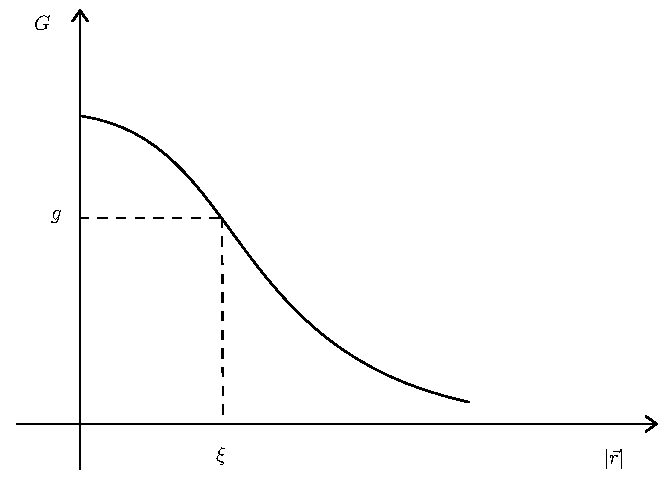
\includegraphics[width=0.6\textwidth]{./img/1.pdf}
\caption{\label{fig:5_1} Plot of the  two-point correlation function, \( G \).}
\end{figure}

\noindent Rearranging the terms, we obtain
\begin{equation}
  \frac{k_B T \chi _T}{V} \leq g \xi ^3
\end{equation}
Hence, if \( \chi _T \) diverges at the critical point it implies \( \xi \rightarrow \infty  \).

In particular, one can see that for \( H=0 \) and \( T \rightarrow T_c^\pm \):
\begin{equation}
  \xi _\pm (T,H=0) \sim \abs{t}^{- \nu _\pm}
  \label{eq:5_2}
\end{equation}
where \( \nu _+ = \nu _- = \nu  \) is the \textbf{Correlation Length Critical Exponent}.
\begin{remark}
It does not derive from thermodynamic considerations, as it is due to the collective behaviour of the units.
\end{remark}
\noindent Scaling is often used as the most general definition of a critical point. 

One can also show that at \( T=T_c \) (i.e. \( t=0 \))
\begin{equation}
  G_c (r) \sim \frac{1}{r^{d-2+\eta }}
\end{equation}
where \( \eta  \) is the correlation critical exponent.
\begin{remark}
The formula is a power law decay instead than exponential.
\end{remark}

\subsection{Critical opalescence: experimental evidence of correlation length divergence}
Microscopic correlations can be proved by \textit{scattering experiments}. For instance, near the critical liquid-gas mixture, the fluid appears "milky", while away from $T_c$ it is transparent. This means that the system is diffusing light, which has $\lambda=500nm$ though, which is much larger than typical atomic distances ($a \approx 1nm$). The scattering of light is caused by density fluctuations, that need to be correlated over long distance to make $\xi$ comparable to $\lambda$.

\section{Finite size effects and phase transitions}
Actually, the thermodynamic limit is a mathematical trick and in real systems it is never reached. Is it then physically relevant?

If we had instruments with \emph{infinite} precision each change of the physical properties of a system would occur within a finite range, therefore we would observe a smooth crossover instead than a singularity. In this respect, the notion of correlation length \( \xi  \) is extremely important.

To illustrate this point, let us consider the gas-liquid system in proximity of its critical point (\( T \sim T_c \) ). If we approach \( T_c \) from the gas phase, there will be fluctuations of \( \rho  \) with respect to \( \rho _G \), \( \Delta \rho = \rho - \rho _G \), due to the presence of denser droplets (liquid) in the continuum gas phase.
These droplets will have different diameters, but the average size would be \( \xi  \), where it is the typical size of the liquid droplets.
Clearly \( \xi = \xi [T] \) and, in proximity of the critical point \( \xi  \overset{t \rightarrow 0}{\sim } \abs{t}^{-\nu }   \).

On the other hand, in a finite system, \( \xi  \) cannot diverge since is bounded above, \( \xi \le L \), where \( L \) is the linear system size.

As \( T \rightarrow T_c \), where \( \xi  \) should be larger than the system size, the behaviour of the system should deviate from the one expected by the theory that is obtained in the limit \( L \rightarrow \infty  \). How far the real system would be from the critical point \( t=0 \) where singularities develop? Let us try to give an estimate of this deviation.

 Let us consider a system of size \( L = \SI{1}{\cm}  \) and
\begin{equation*}
  t \equiv (T-T_c)/T_c, \qquad \xi \sim \xi _0 t^{-\nu }
\end{equation*}
Let us assume that the lattice distance is \( \xi _0 = \SI{10}{\angstrom}  \). Hence,
 \begin{equation}
   t \sim \qty(\frac{\xi }{\xi _0})^{-1/\nu } \sim \qty(\frac{L}{\SI{10}{\angstrom} })^{-1/\nu } \sim (10^{7})^{-1/\nu }
 \end{equation}
In the next chapters, we will see that \( \nu < 1 \) and close to \( 1/2 \), hence:
\begin{equation*}
  t \sim (10^{7})^{-2 } = 10^{-14}
\end{equation*}
Therefore we have \( t \approx 10^{-14} \)  as a distance from \( T_c \).

This estimate suggests that the experimental instrument that measures temperature must have a precision of \( 10^{-14} \)  to see deviations from the results obtained in the thermodynamic limit.


\clearpage

\section{Numerical simulations and phase transitions}

In this case, the size \( L \) of the simulated system is few multiples of \( \xi _0 \) and the finite-size effects of the simulated data can strongly affect the location and the scaling laws of the phase transition under numerical investigation.
Finite size scaling analysis of the numerical data is needed.

\begin{figure}[h!]
\centering
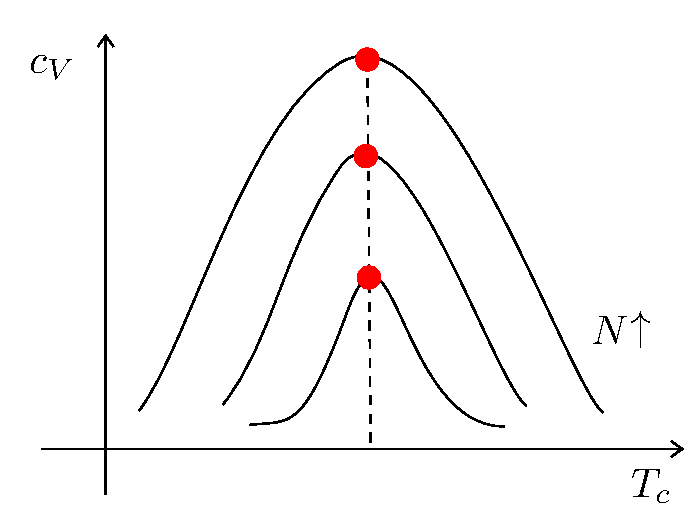
\includegraphics[width=0.5\textwidth]{./img/2.pdf}
\caption{\label{fig:5_2} \( (T_c,C_V) \) plot at different \( N \).}
\end{figure}


We can find the critical point by doing Montecarlo simulation. Supposing a Montecarlo simulation of a Ising model, for which there is no an analytic solution and compute the energy.
Try to extrapolate for example the position of the peak as \emph{N} increases. If we start to see the behaviour, something is happening.
There are two approaches we can use.

 The first approach is studying the system by looking for all the details. An example could be a protein, that interact with other proteins; in this case we can look at all the electrons (or atoms). Nevertheless, even if we thought at the simple protein that exists, there would be a lot of degrees of freedom.

  For doing a simulation, if we are interested in long time behaviour and in large scale behaviour, details are not important. What it is important are symmetries, ranges of interaction. Therefore, we can forget about all the details. We can introduce the effective potentials as Van der Waals or Lenard Jones potential and studying collective effects. This is the second approach.






















\end{document}
